\documentclass[twoside]{book}

% Packages required by doxygen
\usepackage{fixltx2e}
\usepackage{calc}
\usepackage{doxygen}
\usepackage[export]{adjustbox} % also loads graphicx
\usepackage{graphicx}
\usepackage[utf8]{inputenc}
\usepackage{makeidx}
\usepackage{multicol}
\usepackage{multirow}
\PassOptionsToPackage{warn}{textcomp}
\usepackage{textcomp}
\usepackage[nointegrals]{wasysym}
\usepackage[table]{xcolor}

% Font selection
\usepackage[T1]{fontenc}
\usepackage[scaled=.90]{helvet}
\usepackage{courier}
\usepackage{amssymb}
\usepackage{sectsty}
\renewcommand{\familydefault}{\sfdefault}
\allsectionsfont{%
  \fontseries{bc}\selectfont%
  \color{darkgray}%
}
\renewcommand{\DoxyLabelFont}{%
  \fontseries{bc}\selectfont%
  \color{darkgray}%
}
\newcommand{\+}{\discretionary{\mbox{\scriptsize$\hookleftarrow$}}{}{}}

% Page & text layout
\usepackage{geometry}
\geometry{%
  a4paper,%
  top=2.5cm,%
  bottom=2.5cm,%
  left=2.5cm,%
  right=2.5cm%
}
\tolerance=750
\hfuzz=15pt
\hbadness=750
\setlength{\emergencystretch}{15pt}
\setlength{\parindent}{0cm}
\setlength{\parskip}{3ex plus 2ex minus 2ex}
\makeatletter
\renewcommand{\paragraph}{%
  \@startsection{paragraph}{4}{0ex}{-1.0ex}{1.0ex}{%
    \normalfont\normalsize\bfseries\SS@parafont%
  }%
}
\renewcommand{\subparagraph}{%
  \@startsection{subparagraph}{5}{0ex}{-1.0ex}{1.0ex}{%
    \normalfont\normalsize\bfseries\SS@subparafont%
  }%
}
\makeatother

% Headers & footers
\usepackage{fancyhdr}
\pagestyle{fancyplain}
\fancyhead[LE]{\fancyplain{}{\bfseries\thepage}}
\fancyhead[CE]{\fancyplain{}{}}
\fancyhead[RE]{\fancyplain{}{\bfseries\leftmark}}
\fancyhead[LO]{\fancyplain{}{\bfseries\rightmark}}
\fancyhead[CO]{\fancyplain{}{}}
\fancyhead[RO]{\fancyplain{}{\bfseries\thepage}}
\fancyfoot[LE]{\fancyplain{}{}}
\fancyfoot[CE]{\fancyplain{}{}}
\fancyfoot[RE]{\fancyplain{}{\bfseries\scriptsize Generated by Doxygen }}
\fancyfoot[LO]{\fancyplain{}{\bfseries\scriptsize Generated by Doxygen }}
\fancyfoot[CO]{\fancyplain{}{}}
\fancyfoot[RO]{\fancyplain{}{}}
\renewcommand{\footrulewidth}{0.4pt}
\renewcommand{\chaptermark}[1]{%
  \markboth{#1}{}%
}
\renewcommand{\sectionmark}[1]{%
  \markright{\thesection\ #1}%
}

% Indices & bibliography
\usepackage{natbib}
\usepackage[titles]{tocloft}
\setcounter{tocdepth}{3}
\setcounter{secnumdepth}{5}
\makeindex

% Hyperlinks (required, but should be loaded last)
\usepackage{ifpdf}
\ifpdf
  \usepackage[pdftex,pagebackref=true]{hyperref}
\else
  \usepackage[ps2pdf,pagebackref=true]{hyperref}
\fi
\hypersetup{%
  colorlinks=true,%
  linkcolor=blue,%
  citecolor=blue,%
  unicode%
}

% Custom commands
\newcommand{\clearemptydoublepage}{%
  \newpage{\pagestyle{empty}\cleardoublepage}%
}

\usepackage{caption}
\captionsetup{labelsep=space,justification=centering,font={bf},singlelinecheck=off,skip=4pt,position=top}

%===== C O N T E N T S =====

\begin{document}

% Titlepage & ToC
\hypersetup{pageanchor=false,
             bookmarksnumbered=true,
             pdfencoding=unicode
            }
\pagenumbering{alph}
\begin{titlepage}
\vspace*{7cm}
\begin{center}%
{\Large lab 2 indexators documentation }\\
\vspace*{1cm}
{\large Generated by Doxygen 1.8.12}\\
\end{center}
\end{titlepage}
\clearemptydoublepage
\pagenumbering{roman}
\tableofcontents
\clearemptydoublepage
\pagenumbering{arabic}
\hypersetup{pageanchor=true}

%--- Begin generated contents ---
\chapter{Namespace Index}
\section{Packages}
Here are the packages with brief descriptions (if available)\+:\begin{DoxyCompactList}
\item\contentsline{section}{\hyperlink{namespace_c_sharp_lab__1}{C\+Sharp\+Lab\+\_\+1} }{\pageref{namespace_c_sharp_lab__1}}{}
\end{DoxyCompactList}

\chapter{Class Index}
\section{Class List}
Here are the classes, structs, unions and interfaces with brief descriptions\+:\begin{DoxyCompactList}
\item\contentsline{section}{\hyperlink{class_c_sharp_lab2_1_1_int_array}{C\+Sharp\+Lab2.\+Int\+Array} \\*Клас цілочисельного масиву }{\pageref{class_c_sharp_lab2_1_1_int_array}}{}
\item\contentsline{section}{\hyperlink{class_c_sharp_lab2_1_1_program}{C\+Sharp\+Lab2.\+Program} }{\pageref{class_c_sharp_lab2_1_1_program}}{}
\end{DoxyCompactList}

\chapter{File Index}
\section{File List}
Here is a list of all files with brief descriptions\+:\begin{DoxyCompactList}
\item\contentsline{section}{D\+:/\+C\+Sharp/7\+\_\+\+Doroshenko\+\_\+forms2\+\_\+is52/7\+\_\+\+Doroshenko\+\_\+forms2\+\_\+is52/\hyperlink{_estimate_8cs}{Estimate.\+cs} }{\pageref{_estimate_8cs}}{}
\item\contentsline{section}{D\+:/\+C\+Sharp/7\+\_\+\+Doroshenko\+\_\+forms2\+\_\+is52/7\+\_\+\+Doroshenko\+\_\+forms2\+\_\+is52/\hyperlink{_estimate_8_designer_8cs}{Estimate.\+Designer.\+cs} }{\pageref{_estimate_8_designer_8cs}}{}
\item\contentsline{section}{D\+:/\+C\+Sharp/7\+\_\+\+Doroshenko\+\_\+forms2\+\_\+is52/7\+\_\+\+Doroshenko\+\_\+forms2\+\_\+is52/\hyperlink{_form1_8cs}{Form1.\+cs} }{\pageref{_form1_8cs}}{}
\item\contentsline{section}{D\+:/\+C\+Sharp/7\+\_\+\+Doroshenko\+\_\+forms2\+\_\+is52/7\+\_\+\+Doroshenko\+\_\+forms2\+\_\+is52/\hyperlink{_form1_8_designer_8cs}{Form1.\+Designer.\+cs} }{\pageref{_form1_8_designer_8cs}}{}
\item\contentsline{section}{D\+:/\+C\+Sharp/7\+\_\+\+Doroshenko\+\_\+forms2\+\_\+is52/7\+\_\+\+Doroshenko\+\_\+forms2\+\_\+is52/\hyperlink{_form2_8cs}{Form2.\+cs} }{\pageref{_form2_8cs}}{}
\item\contentsline{section}{D\+:/\+C\+Sharp/7\+\_\+\+Doroshenko\+\_\+forms2\+\_\+is52/7\+\_\+\+Doroshenko\+\_\+forms2\+\_\+is52/\hyperlink{_form2_8_designer_8cs}{Form2.\+Designer.\+cs} }{\pageref{_form2_8_designer_8cs}}{}
\item\contentsline{section}{D\+:/\+C\+Sharp/7\+\_\+\+Doroshenko\+\_\+forms2\+\_\+is52/7\+\_\+\+Doroshenko\+\_\+forms2\+\_\+is52/\hyperlink{_form3_8cs}{Form3.\+cs} }{\pageref{_form3_8cs}}{}
\item\contentsline{section}{D\+:/\+C\+Sharp/7\+\_\+\+Doroshenko\+\_\+forms2\+\_\+is52/7\+\_\+\+Doroshenko\+\_\+forms2\+\_\+is52/\hyperlink{_form3_8_designer_8cs}{Form3.\+Designer.\+cs} }{\pageref{_form3_8_designer_8cs}}{}
\item\contentsline{section}{D\+:/\+C\+Sharp/7\+\_\+\+Doroshenko\+\_\+forms2\+\_\+is52/7\+\_\+\+Doroshenko\+\_\+forms2\+\_\+is52/\hyperlink{_individual_8cs}{Individual.\+cs} }{\pageref{_individual_8cs}}{}
\item\contentsline{section}{D\+:/\+C\+Sharp/7\+\_\+\+Doroshenko\+\_\+forms2\+\_\+is52/7\+\_\+\+Doroshenko\+\_\+forms2\+\_\+is52/\hyperlink{_individual_8_designer_8cs}{Individual.\+Designer.\+cs} }{\pageref{_individual_8_designer_8cs}}{}
\item\contentsline{section}{D\+:/\+C\+Sharp/7\+\_\+\+Doroshenko\+\_\+forms2\+\_\+is52/7\+\_\+\+Doroshenko\+\_\+forms2\+\_\+is52/\hyperlink{_program_8cs}{Program.\+cs} }{\pageref{_program_8cs}}{}
\item\contentsline{section}{D\+:/\+C\+Sharp/7\+\_\+\+Doroshenko\+\_\+forms2\+\_\+is52/7\+\_\+\+Doroshenko\+\_\+forms2\+\_\+is52/\hyperlink{_task__1_8cs}{Task\+\_\+1.\+cs} }{\pageref{_task__1_8cs}}{}
\item\contentsline{section}{D\+:/\+C\+Sharp/7\+\_\+\+Doroshenko\+\_\+forms2\+\_\+is52/7\+\_\+\+Doroshenko\+\_\+forms2\+\_\+is52/\hyperlink{_task__1_8_designer_8cs}{Task\+\_\+1.\+Designer.\+cs} }{\pageref{_task__1_8_designer_8cs}}{}
\item\contentsline{section}{D\+:/\+C\+Sharp/7\+\_\+\+Doroshenko\+\_\+forms2\+\_\+is52/7\+\_\+\+Doroshenko\+\_\+forms2\+\_\+is52/\hyperlink{_task__2_8cs}{Task\+\_\+2.\+cs} }{\pageref{_task__2_8cs}}{}
\item\contentsline{section}{D\+:/\+C\+Sharp/7\+\_\+\+Doroshenko\+\_\+forms2\+\_\+is52/7\+\_\+\+Doroshenko\+\_\+forms2\+\_\+is52/\hyperlink{_task__2_8_designer_8cs}{Task\+\_\+2.\+Designer.\+cs} }{\pageref{_task__2_8_designer_8cs}}{}
\item\contentsline{section}{D\+:/\+C\+Sharp/7\+\_\+\+Doroshenko\+\_\+forms2\+\_\+is52/7\+\_\+\+Doroshenko\+\_\+forms2\+\_\+is52/\hyperlink{_task__3_8cs}{Task\+\_\+3.\+cs} }{\pageref{_task__3_8cs}}{}
\item\contentsline{section}{D\+:/\+C\+Sharp/7\+\_\+\+Doroshenko\+\_\+forms2\+\_\+is52/7\+\_\+\+Doroshenko\+\_\+forms2\+\_\+is52/\hyperlink{_task__3_8_designer_8cs}{Task\+\_\+3.\+Designer.\+cs} }{\pageref{_task__3_8_designer_8cs}}{}
\item\contentsline{section}{D\+:/\+C\+Sharp/7\+\_\+\+Doroshenko\+\_\+forms2\+\_\+is52/7\+\_\+\+Doroshenko\+\_\+forms2\+\_\+is52/\hyperlink{_task__4_8cs}{Task\+\_\+4.\+cs} }{\pageref{_task__4_8cs}}{}
\item\contentsline{section}{D\+:/\+C\+Sharp/7\+\_\+\+Doroshenko\+\_\+forms2\+\_\+is52/7\+\_\+\+Doroshenko\+\_\+forms2\+\_\+is52/\hyperlink{_task__4_8_designer_8cs}{Task\+\_\+4.\+Designer.\+cs} }{\pageref{_task__4_8_designer_8cs}}{}
\item\contentsline{section}{D\+:/\+C\+Sharp/7\+\_\+\+Doroshenko\+\_\+forms2\+\_\+is52/7\+\_\+\+Doroshenko\+\_\+forms2\+\_\+is52/\hyperlink{_task__5_8cs}{Task\+\_\+5.\+cs} }{\pageref{_task__5_8cs}}{}
\item\contentsline{section}{D\+:/\+C\+Sharp/7\+\_\+\+Doroshenko\+\_\+forms2\+\_\+is52/7\+\_\+\+Doroshenko\+\_\+forms2\+\_\+is52/\hyperlink{_task__5_8_designer_8cs}{Task\+\_\+5.\+Designer.\+cs} }{\pageref{_task__5_8_designer_8cs}}{}
\item\contentsline{section}{D\+:/\+C\+Sharp/7\+\_\+\+Doroshenko\+\_\+forms2\+\_\+is52/7\+\_\+\+Doroshenko\+\_\+forms2\+\_\+is52/\hyperlink{_task__6_8cs}{Task\+\_\+6.\+cs} }{\pageref{_task__6_8cs}}{}
\item\contentsline{section}{D\+:/\+C\+Sharp/7\+\_\+\+Doroshenko\+\_\+forms2\+\_\+is52/7\+\_\+\+Doroshenko\+\_\+forms2\+\_\+is52/\hyperlink{_task__6_8_designer_8cs}{Task\+\_\+6.\+Designer.\+cs} }{\pageref{_task__6_8_designer_8cs}}{}
\item\contentsline{section}{D\+:/\+C\+Sharp/7\+\_\+\+Doroshenko\+\_\+forms2\+\_\+is52/7\+\_\+\+Doroshenko\+\_\+forms2\+\_\+is52/\hyperlink{_task__7_8cs}{Task\+\_\+7.\+cs} }{\pageref{_task__7_8cs}}{}
\item\contentsline{section}{D\+:/\+C\+Sharp/7\+\_\+\+Doroshenko\+\_\+forms2\+\_\+is52/7\+\_\+\+Doroshenko\+\_\+forms2\+\_\+is52/\hyperlink{_task__7_8_designer_8cs}{Task\+\_\+7.\+Designer.\+cs} }{\pageref{_task__7_8_designer_8cs}}{}
\item\contentsline{section}{D\+:/\+C\+Sharp/7\+\_\+\+Doroshenko\+\_\+forms2\+\_\+is52/7\+\_\+\+Doroshenko\+\_\+forms2\+\_\+is52/\hyperlink{_task__8_8cs}{Task\+\_\+8.\+cs} }{\pageref{_task__8_8cs}}{}
\item\contentsline{section}{D\+:/\+C\+Sharp/7\+\_\+\+Doroshenko\+\_\+forms2\+\_\+is52/7\+\_\+\+Doroshenko\+\_\+forms2\+\_\+is52/\hyperlink{_task__8_8_designer_8cs}{Task\+\_\+8.\+Designer.\+cs} }{\pageref{_task__8_8_designer_8cs}}{}
\item\contentsline{section}{D\+:/\+C\+Sharp/7\+\_\+\+Doroshenko\+\_\+forms2\+\_\+is52/7\+\_\+\+Doroshenko\+\_\+forms2\+\_\+is52/\hyperlink{_task__9_8cs}{Task\+\_\+9.\+cs} }{\pageref{_task__9_8cs}}{}
\item\contentsline{section}{D\+:/\+C\+Sharp/7\+\_\+\+Doroshenko\+\_\+forms2\+\_\+is52/7\+\_\+\+Doroshenko\+\_\+forms2\+\_\+is52/\hyperlink{_task__9_8_designer_8cs}{Task\+\_\+9.\+Designer.\+cs} }{\pageref{_task__9_8_designer_8cs}}{}
\end{DoxyCompactList}

\chapter{Namespace Documentation}
\hypertarget{namespace_c_sharp_lab2}{}\section{C\+Sharp\+Lab2 Namespace Reference}
\label{namespace_c_sharp_lab2}\index{C\+Sharp\+Lab2@{C\+Sharp\+Lab2}}
\subsection*{Classes}
\begin{DoxyCompactItemize}
\item 
class \hyperlink{class_c_sharp_lab2_1_1_int_array}{Int\+Array}
\begin{DoxyCompactList}\small\item\em Клас цілочисельного масиву \end{DoxyCompactList}\item 
class \hyperlink{class_c_sharp_lab2_1_1_program}{Program}
\end{DoxyCompactItemize}

\chapter{Class Documentation}
\hypertarget{class_c_sharp_lab2_1_1_int_array}{}\section{C\+Sharp\+Lab2.\+Int\+Array Class Reference}
\label{class_c_sharp_lab2_1_1_int_array}\index{C\+Sharp\+Lab2.\+Int\+Array@{C\+Sharp\+Lab2.\+Int\+Array}}


Клас цілочисельного масиву  




Collaboration diagram for C\+Sharp\+Lab2.\+Int\+Array\+:
\nopagebreak
\begin{figure}[H]
\begin{center}
\leavevmode
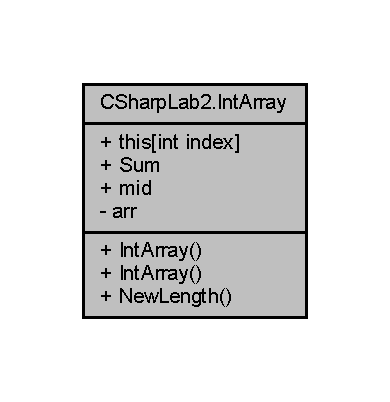
\includegraphics[width=187pt]{class_c_sharp_lab2_1_1_int_array__coll__graph}
\end{center}
\end{figure}
\subsection*{Public Member Functions}
\begin{DoxyCompactItemize}
\item 
\hyperlink{class_c_sharp_lab2_1_1_int_array_a3fe8a5d200583c1c345b4af4e14024be}{Int\+Array} ()
\begin{DoxyCompactList}\small\item\em Конструктор за замовчуванням \end{DoxyCompactList}\item 
\hyperlink{class_c_sharp_lab2_1_1_int_array_acc7eb5c0179289e1d64e791ee0ee5cce}{Int\+Array} (int size)
\begin{DoxyCompactList}\small\item\em Конструктор ініціалізації \end{DoxyCompactList}\item 
int \hyperlink{class_c_sharp_lab2_1_1_int_array_abe62d3588deef8d7e98ed5b3fd18e6fb}{New\+Length} ()
\begin{DoxyCompactList}\small\item\em довжина \end{DoxyCompactList}\end{DoxyCompactItemize}
\subsection*{Properties}
\begin{DoxyCompactItemize}
\item 
int \hyperlink{class_c_sharp_lab2_1_1_int_array_a42f8a711f5fbeba620b137326bbc241d}{this\mbox{[}int index\mbox{]}}\hspace{0.3cm}{\ttfamily  \mbox{[}get, set\mbox{]}}
\begin{DoxyCompactList}\small\item\em Індексатор \end{DoxyCompactList}\item 
int \hyperlink{class_c_sharp_lab2_1_1_int_array_a8a753df2be5385be3b9dcf8cdf70d7fb}{Sum}\hspace{0.3cm}{\ttfamily  \mbox{[}get\mbox{]}}
\begin{DoxyCompactList}\small\item\em Сума всіх елементів масиву \end{DoxyCompactList}\item 
float \hyperlink{class_c_sharp_lab2_1_1_int_array_abb9c31974804db308f3628d1d98ece91}{mid}\hspace{0.3cm}{\ttfamily  \mbox{[}get\mbox{]}}
\begin{DoxyCompactList}\small\item\em середнє арифметичне \end{DoxyCompactList}\end{DoxyCompactItemize}
\subsection*{Private Attributes}
\begin{DoxyCompactItemize}
\item 
int \mbox{[}$\,$\mbox{]} \hyperlink{class_c_sharp_lab2_1_1_int_array_adfe65a25352fc485dfd771e03c9b9362}{arr}
\begin{DoxyCompactList}\small\item\em масив чисел \end{DoxyCompactList}\end{DoxyCompactItemize}


\subsection{Detailed Description}
Клас цілочисельного масиву 



\subsection{Constructor \& Destructor Documentation}
\hypertarget{class_c_sharp_lab2_1_1_int_array_a3fe8a5d200583c1c345b4af4e14024be}{}\label{class_c_sharp_lab2_1_1_int_array_a3fe8a5d200583c1c345b4af4e14024be} 
\index{C\+Sharp\+Lab2\+::\+Int\+Array@{C\+Sharp\+Lab2\+::\+Int\+Array}!Int\+Array@{Int\+Array}}
\index{Int\+Array@{Int\+Array}!C\+Sharp\+Lab2\+::\+Int\+Array@{C\+Sharp\+Lab2\+::\+Int\+Array}}
\subsubsection{\texorpdfstring{Int\+Array()}{IntArray()}\hspace{0.1cm}{\footnotesize\ttfamily [1/2]}}
{\footnotesize\ttfamily C\+Sharp\+Lab2.\+Int\+Array.\+Int\+Array (\begin{DoxyParamCaption}{ }\end{DoxyParamCaption})\hspace{0.3cm}{\ttfamily [inline]}}



Конструктор за замовчуванням 

\hypertarget{class_c_sharp_lab2_1_1_int_array_acc7eb5c0179289e1d64e791ee0ee5cce}{}\label{class_c_sharp_lab2_1_1_int_array_acc7eb5c0179289e1d64e791ee0ee5cce} 
\index{C\+Sharp\+Lab2\+::\+Int\+Array@{C\+Sharp\+Lab2\+::\+Int\+Array}!Int\+Array@{Int\+Array}}
\index{Int\+Array@{Int\+Array}!C\+Sharp\+Lab2\+::\+Int\+Array@{C\+Sharp\+Lab2\+::\+Int\+Array}}
\subsubsection{\texorpdfstring{Int\+Array()}{IntArray()}\hspace{0.1cm}{\footnotesize\ttfamily [2/2]}}
{\footnotesize\ttfamily C\+Sharp\+Lab2.\+Int\+Array.\+Int\+Array (\begin{DoxyParamCaption}\item[{int}]{size }\end{DoxyParamCaption})\hspace{0.3cm}{\ttfamily [inline]}}



Конструктор ініціалізації 


\begin{DoxyParams}{Parameters}
{\em size} & Розмір масиву\\
\hline
\end{DoxyParams}


\subsection{Member Function Documentation}
\hypertarget{class_c_sharp_lab2_1_1_int_array_abe62d3588deef8d7e98ed5b3fd18e6fb}{}\label{class_c_sharp_lab2_1_1_int_array_abe62d3588deef8d7e98ed5b3fd18e6fb} 
\index{C\+Sharp\+Lab2\+::\+Int\+Array@{C\+Sharp\+Lab2\+::\+Int\+Array}!New\+Length@{New\+Length}}
\index{New\+Length@{New\+Length}!C\+Sharp\+Lab2\+::\+Int\+Array@{C\+Sharp\+Lab2\+::\+Int\+Array}}
\subsubsection{\texorpdfstring{New\+Length()}{NewLength()}}
{\footnotesize\ttfamily int C\+Sharp\+Lab2.\+Int\+Array.\+New\+Length (\begin{DoxyParamCaption}{ }\end{DoxyParamCaption})\hspace{0.3cm}{\ttfamily [inline]}}



довжина 

\begin{DoxyReturn}{Returns}
довжину масиву
\end{DoxyReturn}
Here is the caller graph for this function\+:
\nopagebreak
\begin{figure}[H]
\begin{center}
\leavevmode
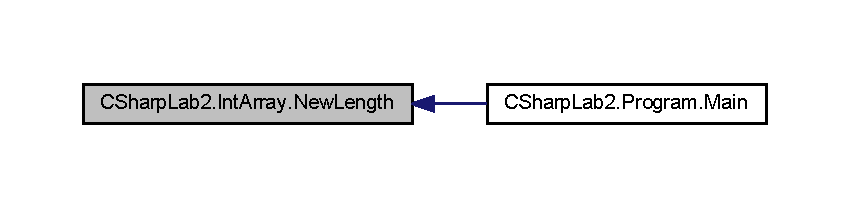
\includegraphics[width=350pt]{class_c_sharp_lab2_1_1_int_array_abe62d3588deef8d7e98ed5b3fd18e6fb_icgraph}
\end{center}
\end{figure}


\subsection{Member Data Documentation}
\hypertarget{class_c_sharp_lab2_1_1_int_array_adfe65a25352fc485dfd771e03c9b9362}{}\label{class_c_sharp_lab2_1_1_int_array_adfe65a25352fc485dfd771e03c9b9362} 
\index{C\+Sharp\+Lab2\+::\+Int\+Array@{C\+Sharp\+Lab2\+::\+Int\+Array}!arr@{arr}}
\index{arr@{arr}!C\+Sharp\+Lab2\+::\+Int\+Array@{C\+Sharp\+Lab2\+::\+Int\+Array}}
\subsubsection{\texorpdfstring{arr}{arr}}
{\footnotesize\ttfamily int \mbox{[}$\,$\mbox{]} C\+Sharp\+Lab2.\+Int\+Array.\+arr\hspace{0.3cm}{\ttfamily [private]}}



масив чисел 



\subsection{Property Documentation}
\hypertarget{class_c_sharp_lab2_1_1_int_array_abb9c31974804db308f3628d1d98ece91}{}\label{class_c_sharp_lab2_1_1_int_array_abb9c31974804db308f3628d1d98ece91} 
\index{C\+Sharp\+Lab2\+::\+Int\+Array@{C\+Sharp\+Lab2\+::\+Int\+Array}!mid@{mid}}
\index{mid@{mid}!C\+Sharp\+Lab2\+::\+Int\+Array@{C\+Sharp\+Lab2\+::\+Int\+Array}}
\subsubsection{\texorpdfstring{mid}{mid}}
{\footnotesize\ttfamily float C\+Sharp\+Lab2.\+Int\+Array.\+mid\hspace{0.3cm}{\ttfamily [get]}}



середнє арифметичне 

\hypertarget{class_c_sharp_lab2_1_1_int_array_a8a753df2be5385be3b9dcf8cdf70d7fb}{}\label{class_c_sharp_lab2_1_1_int_array_a8a753df2be5385be3b9dcf8cdf70d7fb} 
\index{C\+Sharp\+Lab2\+::\+Int\+Array@{C\+Sharp\+Lab2\+::\+Int\+Array}!Sum@{Sum}}
\index{Sum@{Sum}!C\+Sharp\+Lab2\+::\+Int\+Array@{C\+Sharp\+Lab2\+::\+Int\+Array}}
\subsubsection{\texorpdfstring{Sum}{Sum}}
{\footnotesize\ttfamily int C\+Sharp\+Lab2.\+Int\+Array.\+Sum\hspace{0.3cm}{\ttfamily [get]}}



Сума всіх елементів масиву 

\hypertarget{class_c_sharp_lab2_1_1_int_array_a42f8a711f5fbeba620b137326bbc241d}{}\label{class_c_sharp_lab2_1_1_int_array_a42f8a711f5fbeba620b137326bbc241d} 
\index{C\+Sharp\+Lab2\+::\+Int\+Array@{C\+Sharp\+Lab2\+::\+Int\+Array}!this\mbox{[}int index\mbox{]}@{this[int index]}}
\index{this\mbox{[}int index\mbox{]}@{this[int index]}!C\+Sharp\+Lab2\+::\+Int\+Array@{C\+Sharp\+Lab2\+::\+Int\+Array}}
\subsubsection{\texorpdfstring{this[int index]}{this[int index]}}
{\footnotesize\ttfamily int C\+Sharp\+Lab2.\+Int\+Array.\+this\mbox{[}int index\mbox{]}\hspace{0.3cm}{\ttfamily [get]}, {\ttfamily [set]}}



Індексатор 


\begin{DoxyParams}{Parameters}
{\em index} & індекс елемента\\
\hline
\end{DoxyParams}
\begin{DoxyReturn}{Returns}
Значення елмента за вказаним індексом
\end{DoxyReturn}


The documentation for this class was generated from the following file\+:\begin{DoxyCompactItemize}
\item 
\hyperlink{_int_array_8cs}{Int\+Array.\+cs}\end{DoxyCompactItemize}

\hypertarget{class_c_sharp_lab2_1_1_program}{}\section{C\+Sharp\+Lab2.\+Program Class Reference}
\label{class_c_sharp_lab2_1_1_program}\index{C\+Sharp\+Lab2.\+Program@{C\+Sharp\+Lab2.\+Program}}


Collaboration diagram for C\+Sharp\+Lab2.\+Program\+:
\nopagebreak
\begin{figure}[H]
\begin{center}
\leavevmode
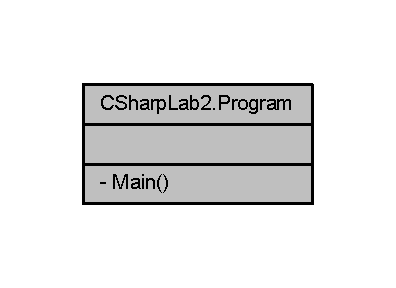
\includegraphics[width=190pt]{class_c_sharp_lab2_1_1_program__coll__graph}
\end{center}
\end{figure}
\subsection*{Static Private Member Functions}
\begin{DoxyCompactItemize}
\item 
static void \hyperlink{class_c_sharp_lab2_1_1_program_ad1384680a182efdc7cf9f8eb73540648}{Main} (string\mbox{[}$\,$\mbox{]} args)
\end{DoxyCompactItemize}


\subsection{Member Function Documentation}
\hypertarget{class_c_sharp_lab2_1_1_program_ad1384680a182efdc7cf9f8eb73540648}{}\label{class_c_sharp_lab2_1_1_program_ad1384680a182efdc7cf9f8eb73540648} 
\index{C\+Sharp\+Lab2\+::\+Program@{C\+Sharp\+Lab2\+::\+Program}!Main@{Main}}
\index{Main@{Main}!C\+Sharp\+Lab2\+::\+Program@{C\+Sharp\+Lab2\+::\+Program}}
\subsubsection{\texorpdfstring{Main()}{Main()}}
{\footnotesize\ttfamily static void C\+Sharp\+Lab2.\+Program.\+Main (\begin{DoxyParamCaption}\item[{string \mbox{[}$\,$\mbox{]}}]{args }\end{DoxyParamCaption})\hspace{0.3cm}{\ttfamily [inline]}, {\ttfamily [static]}, {\ttfamily [private]}}

Here is the call graph for this function\+:
\nopagebreak
\begin{figure}[H]
\begin{center}
\leavevmode
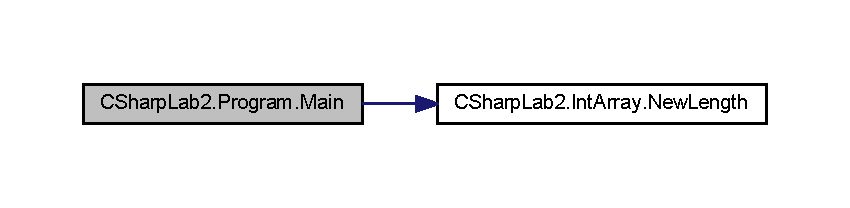
\includegraphics[width=350pt]{class_c_sharp_lab2_1_1_program_ad1384680a182efdc7cf9f8eb73540648_cgraph}
\end{center}
\end{figure}


The documentation for this class was generated from the following file\+:\begin{DoxyCompactItemize}
\item 
\hyperlink{_program_8cs}{Program.\+cs}\end{DoxyCompactItemize}

\chapter{File Documentation}
\hypertarget{_int_array_8cs}{}\section{Int\+Array.\+cs File Reference}
\label{_int_array_8cs}\index{Int\+Array.\+cs@{Int\+Array.\+cs}}
\subsection*{Classes}
\begin{DoxyCompactItemize}
\item 
class \hyperlink{class_c_sharp_lab2_1_1_int_array}{C\+Sharp\+Lab2.\+Int\+Array}
\begin{DoxyCompactList}\small\item\em Клас цілочисельного масиву \end{DoxyCompactList}\end{DoxyCompactItemize}
\subsection*{Namespaces}
\begin{DoxyCompactItemize}
\item 
namespace \hyperlink{namespace_c_sharp_lab2}{C\+Sharp\+Lab2}
\end{DoxyCompactItemize}

\hypertarget{_program_8cs}{}\section{Program.\+cs File Reference}
\label{_program_8cs}\index{Program.\+cs@{Program.\+cs}}
\subsection*{Classes}
\begin{DoxyCompactItemize}
\item 
class \hyperlink{class_c_sharp_lab2_1_1_program}{C\+Sharp\+Lab2.\+Program}
\end{DoxyCompactItemize}
\subsection*{Namespaces}
\begin{DoxyCompactItemize}
\item 
namespace \hyperlink{namespace_c_sharp_lab2}{C\+Sharp\+Lab2}
\end{DoxyCompactItemize}

%--- End generated contents ---

% Index
\backmatter
\newpage
\phantomsection
\clearemptydoublepage
\addcontentsline{toc}{chapter}{Index}
\printindex

\end{document}
